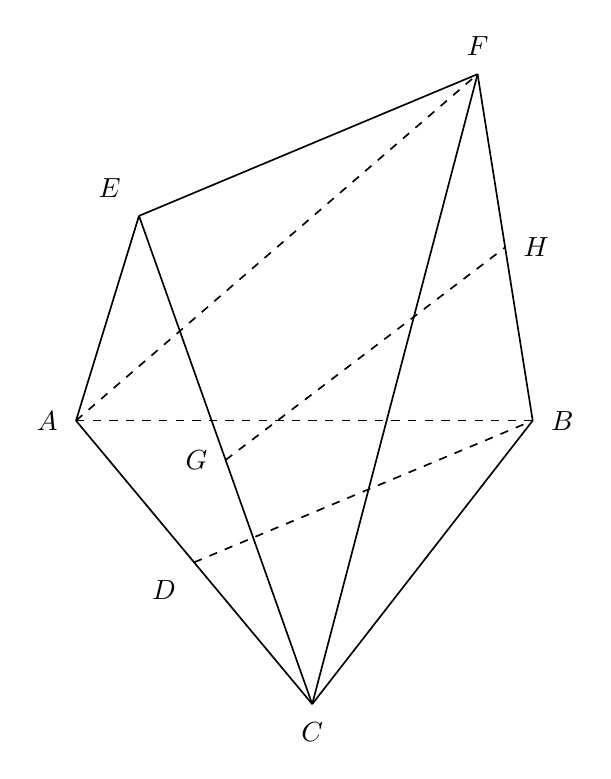
\begin{tikzpicture}[x=1cm,y=1cm,line width=.6pt,font=\normalsize]
\coordinate (A) at (-3.4,1.0);
\coordinate (B) at (2.4,1.0);
\coordinate (C) at (-0.4,-2.6);
\coordinate (D) at (-1.9000000000,-0.8000000000);
\coordinate (E) at (-2.6,3.6);
\coordinate (F) at (1.7000000000,5.4000000000);
\coordinate (G) at (-1.5000000000,0.5000000000);
\coordinate (H) at (2.0500000000,3.2000000000);
% solid visible edges
\draw[solid] (A)--(E);
\draw[solid] (E)--(F);
\draw[solid] (F)--(B);
\draw[solid] (B)--(C);
\draw[solid] (C)--(A);
\draw[solid] (E)--(C);
\draw[solid] (F)--(C);
% dashed hidden edges
\draw[dashed] (A)--(F);
\draw[dashed] (A)--(B);
\draw[dashed] (D)--(B);
\draw[dashed] (G)--(H);
\node[left,xshift=-3pt] at (A) {$A$};
\node[right,xshift=3pt] at (B) {$B$};
\node[below,yshift=-3pt] at (C) {$C$};
\node[below left,xshift=-3.0pt,yshift=-3.0pt] at (D) {$D$};
\node[above left,xshift=-3.0pt,yshift=3.0pt] at (E) {$E$};
\node[above,yshift=3pt] at (F) {$F$};
\node[left,xshift=-3pt] at (G) {$G$};
\node[right,xshift=3pt] at (H) {$H$};
\end{tikzpicture}